\section{Experiments}
\label{sec:experiments}

In this section, we first explore if ViTs trained with different objectives all have artifacts. Then, we evaluate the effectiveness of our generalizable denoiser on dense prediction tasks. For all experiments, we default to using ViT-\textit{base} models with patch sizes of 14 or 16, depending on the availability of their implementations and model weights in PyTorch Image Models (\texttt{timm} \cite{rw2019timm}). We defer all the implementation details to the appendix.

\subsection{Artifacts in ViTs}

\paragraph{Positional artifacts in different ViTs.}
We visualize feature maps from differently pre-trained ViTs in \cref{fig:teaser}. Among these, DINOv2 \cite{oquab2023dinov2}, a state-of-the-art vision foundation model with excellent performance on downstream tasks, displays clear position-related artifacts. Additionally, DeIT-III \cite{touvron2022deit}, trained with image class labels, and CLIP \cite{radford2021learning}, trained by text-image alignment, also exhibit noticeable artifacts. Furthermore, EVA02 \cite{fang2023eva}, which distills local patch features from a pre-trained CLIP model using masked image modeling, also has clear feature artifacts. In ViTs we have tested, our proposed \ours successfully mitigates these artifacts (``Original features'' \textit{vs.} ``Denoised features'' in \cref{fig:teaser}).


%##################################################################################################
\begin{figure}[t!]
    \centering
    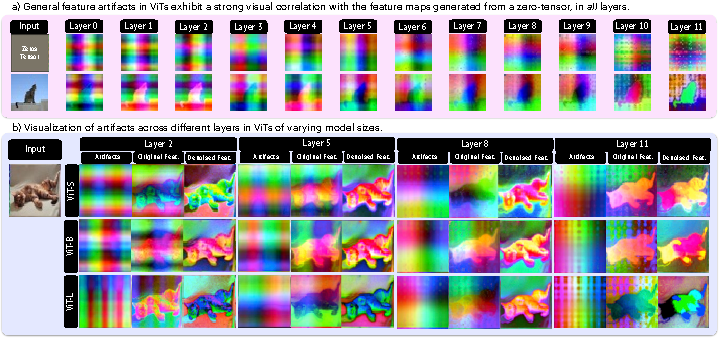
\includegraphics[width=1\linewidth]{figures/fig5_zero_tensors.pdf}
    \caption{\textbf{Visual analysis of ViT output features and denoised features.} (a) Visualizations of the feature maps from all layers of a DINOv2 \cite{oquab2023dinov2} ViT-\textit{base} model. Notably, the artifacts in the feature maps derived from the cat image exhibit a strong visual correlation with those from the zero-tensor inputs. (b) Visualizations of the decomposed artifacts, the original features, and the denoised features across various layers of DINOv2 ViTs. We observe similar patterns in differently-sized models.}
    \label{fig:multilayer}
\end{figure}
%##################################################################################################


\paragraph{Artifacts in different layers.} In \cref{fig:multilayer}, we present a visual analysis of the artifact decomposition across various layers of DINOv2 ViTs of different sizes (b), alongside feature maps generated using only zero-tensors as input (a). Notably, the artifacts decomposed by our \ours show a strong visual resemblance to these zero-tensor-input feature maps. In addition, we observe that the artifacts vary across layers: the shallower layers predominantly exhibit low-frequency patterns, whereas the deeper layers are characterized by high-frequency patterns. Importantly, these patterns are consistent across ViTs of different sizes (\eg, from ViT-\textit{small} to ViT-\textit{large}), diverging from the hypothesis in \cite{darcet2023vision} that only large ViTs would display such patterns.

%Further, \cref{fig:multilayer}-(c) showcases the enhanced similarity of central patches compared to other patches post-denoising. Lastly, we see that the artifacts in feature maps will hurt the K-means clustering accuracy significantly and our \ours addresses this issue. These factors are crucial for dense prediction tasks.
\begin{table*}[t!]
    \centering
    \small
    \caption{\textbf{Comparison of features correlation to spatial positions.} We report the maximal information coefficient (MIC) between grid features and their coordinates.}
    \tablestyle{3.5pt}{1.2}
    \begin{tabular}{l | x{60} | x{60} | x{60}}
                                        & \textbf{Before denoising} & \multicolumn{2}{c}{\textbf{After denoising}}                                         \\

        Method                          & \textbf{Raw features}     & \textbf{Artifacts term $\mathcal{G}$}        & \textbf{Semantics term $\mathcal{F}$} \\
        \shline
        DINOv2 \cite{oquab2023dinov2}   & 0.44                      & 0.54                                         & 0.22                                  \\
        DeiT-III \cite{touvron2022deit} & 0.34                      & 0.32                                         & 0.06                                  \\
        CLIP \cite{radford2021learning} & 0.11                      & 0.14                                         & 0.08                                  \\
    \end{tabular}
    \label{tab:correlation}
\end{table*}
%##################################################################################################


\paragraph{Correlation between artifacts and positions.} Beyond visual qualitative inspection, we aim to quantitatively analyze the correlation between artifacts and their positions. Similar to \cite{voita2023neurons}, we use the maximal information coefficient (MIC) to measure the dependency between grid features and their normalized patch coordinates (See appendix for more details). This metric indicates how much patch features depend on their spatial positions and semantic content. As shown in \cref{tab:correlation}, both the original ViT outputs and the decomposed artifacts exhibit a higher spatial correlation than the denoised semantic features, irrespective of the training methodology employed. These results support our hypothesis about the significant role of positional embeddings in the emergence of artifacts. Note that there is no ``ground-truth'' quantitative metric to to definitively quantify these patterns; hence, our reported numerical results should be viewed as empirical indicators, akin to the ``high-norm'' indicator used in \cite{darcet2023vision}.


\subsection{Evaluation on Downstream Task Performance}

We evaluate our method in dense recognition tasks, including semantic segmentation, monocular depth estimation, object detection, and object discovery. It is important to note that there is no direct competitor for these tasks in our study. Instead, our focus is on comparing the performance of pre-trained ViTs before and after applying our \ours. For all the models in the main experiments, we use 10k denoised samples randomly selected from the VOC2012 and the VOC2007 datasets, excluding their validation samples, to train generalizable denoisers.

\paragraph{Semantic segmentation.} We follow \cite{oquab2023dinov2,darcet2023vision} to evaluate our approach in two semantic segmentation datasets: VOC2012 \cite{pascal-voc-2012}
and ADE20k \cite{zhou2018semantic}, using a linear probing protocol, \ie, a linear layer is trained to predict pixels' class from patch tokens.
\cref{tab:dense_results}
presents the main results. We observe significant and consistent enhancements in all pre-trained ViTs across datasets. Notably, the DINOv2-\textit{giant}, with an 83.0 mIoU on VOC2012 as reported in \cite{oquab2023dinov2}, is outperformed by our \ours-denoised DINOv2-\textit{base} model (84.84 mIoU). This improvement is also evident in the ADE20k dataset, where the DINOv2-\textit{giant} and DINOv2-\textit{large} models attain mIoUs of 49.0 and 47.7, respectively, as reported in \cite{oquab2023dinov2}, while our denoised \textit{base} model achieves a 48.66 mIoU. Remarkably, the \textit{giant} model, which is $\mathbf{13\times}$ larger than the \textit{base} model, is outperformed by or on par with our denoised \textit{base} model. This indicates that the performance gains primarily stem from effective artifact removal rather than the \textit{minor} increase in model parameters of our denoiser network.

Our \ours also increases the performance of the concurrent DINOv2-reg model \cite{darcet2023vision}, where a ViT is trained with dummy learnable register tokens. As evidenced in \cref{tab:dense_results}, our \ours enhances the performance of both DINOv2 ((f1) \textit{vs.} (f2)) and DINOv2-reg ((e1) \textit{vs.} (e2)). When applying \ours only, DINOv2 shows more improvements compared to using registers ((f2) \textit{vs.} (e1)); for instance, DINOv2 denoised by \ours achieves 84.84 mIoU in VOC2012 and 48.66 mIoU in ADE20k, surpassing the performance of DINOv2-reg, which achieves 83.64 mIoU and 48.22 mIoU on the respective benchmarks. Furthermore, \ours can further enhance the performance of DINOv2-reg ((e1) \textit{vs.} (e2)) on both datasets (+0.86 in VOC2012 and +1.12 in ADE20k).
In addition, DINOv2-reg \cite{darcet2023vision} requires retraining entire models from scratch using 142M images, while our approach requires training a single Transformer block using 10k denoised samples.

%##################################################################################################
\begin{table*}[t!]
    \centering
    \small
    \caption{\textbf{Quantitative performance of \ours.} \ours improves differently pre-trained ViTs for dense prediction tasks. We report performance on semantic segmentation (VOC2012, ADE20K) and depth prediction (NYUd) tasks.}
    \tablestyle{3.5pt}{1.2}
    \begin{tabular}{l | x{35}x{35} | x{35}x{35} | x{35}x{35} }
                                                                 & \multicolumn{2}{c|}{VOC2012 Segmentation} & \multicolumn{2}{c|}{ADE20k Segmentation} & \multicolumn{2}{c}{NYUv2 Depth Estimation}                                                     \\
        Method
                                                                 & mIoU($\uparrow$)
                                                                 & mAcc($\uparrow$)
                                                                 & mIoU($\uparrow$)
                                                                 & mAcc($\uparrow$)                          & $\delta_1$($\uparrow$)                   & abs rel($\downarrow$)                                                                          \\
        \shline
        (a1) DINO \cite{caron2021emerging}                       & 63.00                                     & 76.35                                    & 31.03                                      & 40.33          & 73.19          & \textbf{0.1701} \\
        (a2) DINO \cite{caron2021emerging} + \textbf{\ours}      & \textbf{66.22}                            & \textbf{78.14}                           & \textbf{32.40}                             & \textbf{42.01} & \textbf{73.53} & 0.1731          \\
        \hline
        (b1) DeiT-III \cite{touvron2022deit}                     & 70.62                                     & 81.23                                    & 32.73                                      & 42.81          & \textbf{72.16} & \textbf{0.1788} \\
        (b2) DeiT-III \cite{touvron2022deit} + \textbf{\ours}    & \textbf{73.36}                            & \textbf{83.74}                           & \textbf{36.57}                             & \textbf{49.01} & 71.36          & 0.1802          \\
        \hline
        (c1) EVA02 \cite{fang2023eva}                            & 71.52                                     & 82.95                                    & 37.45                                      & 49.74          & 63.68          & 0.1989          \\
        (c2) EVA02 \cite{fang2023eva}  + \textbf{\ours}          & \textbf{73.15}                            & \textbf{83.55}                           & \textbf{37.87}                             & \textbf{49.81} & \textbf{68.52} & \textbf{0.1964} \\
        \hline
        (d1) CLIP \cite{radford2021learning}                     & 77.78                                     & 86.57                                    & 40.51                                      & 52.47          & 73.95          & 0.1679          \\
        (d2) CLIP \cite{radford2021learning} + \textbf{\ours}    & \textbf{79.01}                            & \textbf{87.48}                           & \textbf{41.10}                             & \textbf{53.07} & \textbf{74.61} & \textbf{0.1667} \\
        \hline
        (e1) DINOv2-reg \cite{darcet2023vision}                  & 83.64                                     & 90.67                                    & 48.22                                      & 60.52          & 87.88          & 0.1190          \\
        (e2) DINOv2-reg \cite{darcet2023vision} + \textbf{\ours} & \textbf{84.50}                            & \textbf{91.45}                           & \textbf{49.34}                             & \textbf{61.70} & \textbf{88.26} & \textbf{0.1157} \\
        \hline
        (f1) DINOv2 \cite{oquab2023dinov2}                       & 83.60                                     & 90.82                                    & 47.29                                      & 59.18          & 86.88          & 0.1238          \\
        (f2) DINOv2 \cite{oquab2023dinov2} + \textbf{\ours}      & \textbf{84.84}                            & \textbf{91.70}                           & \textbf{48.66}                             & \textbf{60.24} & \textbf{87.58} & \textbf{0.1200}
    \end{tabular}
    \label{tab:dense_results}
\end{table*}
%##################################################################################################

\paragraph{Depth estimation.} Following \cite{oquab2023dinov2}, we evaluate our method on the NYUv2-Depth dataset \cite{Silberman_ECCV12} using a linear evaluation protocol (more details in appendix). As shown in \cref{tab:dense_results}, our method clearly enhances the performance of most pre-trained ViTs. For context, the DINOv2-\textit{large} model exhibits a 0.01 RMSE improvement over the DINOv2-\textit{base} model with 3.5$\times$ more parameters. Our denoiser achieves similar performance gains with 0.08$\times$ the parameters of the base model. These results highlight our method's efficiency, achieving marked performance gains with minimal increases in parameter count.

%##################################################################################################
\begin{table}[t!]
    \centering
    \small
    \caption{\textbf{Object detection with frozen features.} We report the mAP metric on the VOC object detection benchmark.}
    \tablestyle{3.5pt}{1.2}
    \begin{tabular}{l | y{40} y{50} y{40}  y{40}  y{40} y{40}}
        Method                               & DINOv2 \cite{oquab2023dinov2}
                                             & DINOv2-reg \cite{darcet2023vision}
                                             & CLIP \cite{radford2021learning}
                                             & DeiT-III \cite{touvron2022deit}
                                             & DINO \cite{caron2021emerging}
                                             & EVA02 \cite{fang2022eva}                                                                                                                                                                                                                                                    \\
        \shline
        baseline                             & 81.4                                       & 80.9                                       & 80.9                                       & 75.8                                       & 76.4                                       & 79.4                                       \\
        \baseline{baseline + \textbf{\ours}} & \baseline{\textbf{81.9} \increase{(+0.5)}} & \baseline{\textbf{81.4} \increase{(+0.5)}} & \baseline{\textbf{81.7} \increase{(+0.9)}} & \baseline{\textbf{77.0} \increase{(+1.2)}} & \baseline{\textbf{77.1} \increase{(+0.7)}} & \baseline{\textbf{80.2} \increase{(+0.8)}} \\
    \end{tabular}
    \label{tab:obj_det}
\end{table}
%##################################################################################################

\paragraph{Object detection.} In this experiment, we train ViTDet detectors \cite{li2022exploring} on the frozen features following the Faster RCNN framework \cite{ren2015faster} (more details in appendix). We train all models on the VOC \texttt{trainval07+12} subset and report their mAP metrics on the \texttt{test2007} subset. Results are reported in \cref{tab:obj_det}. Our approach shows consistent improvements over the studied ViTs. Notably, DINOv2-reg \cite{darcet2023vision} shows a slight decrease in object detection performance when compared to the original DINOv2 \cite{oquab2023dinov2}, while our approach improves it.


%##################################################################################################
\begin{figure}[t!]
    \centering
    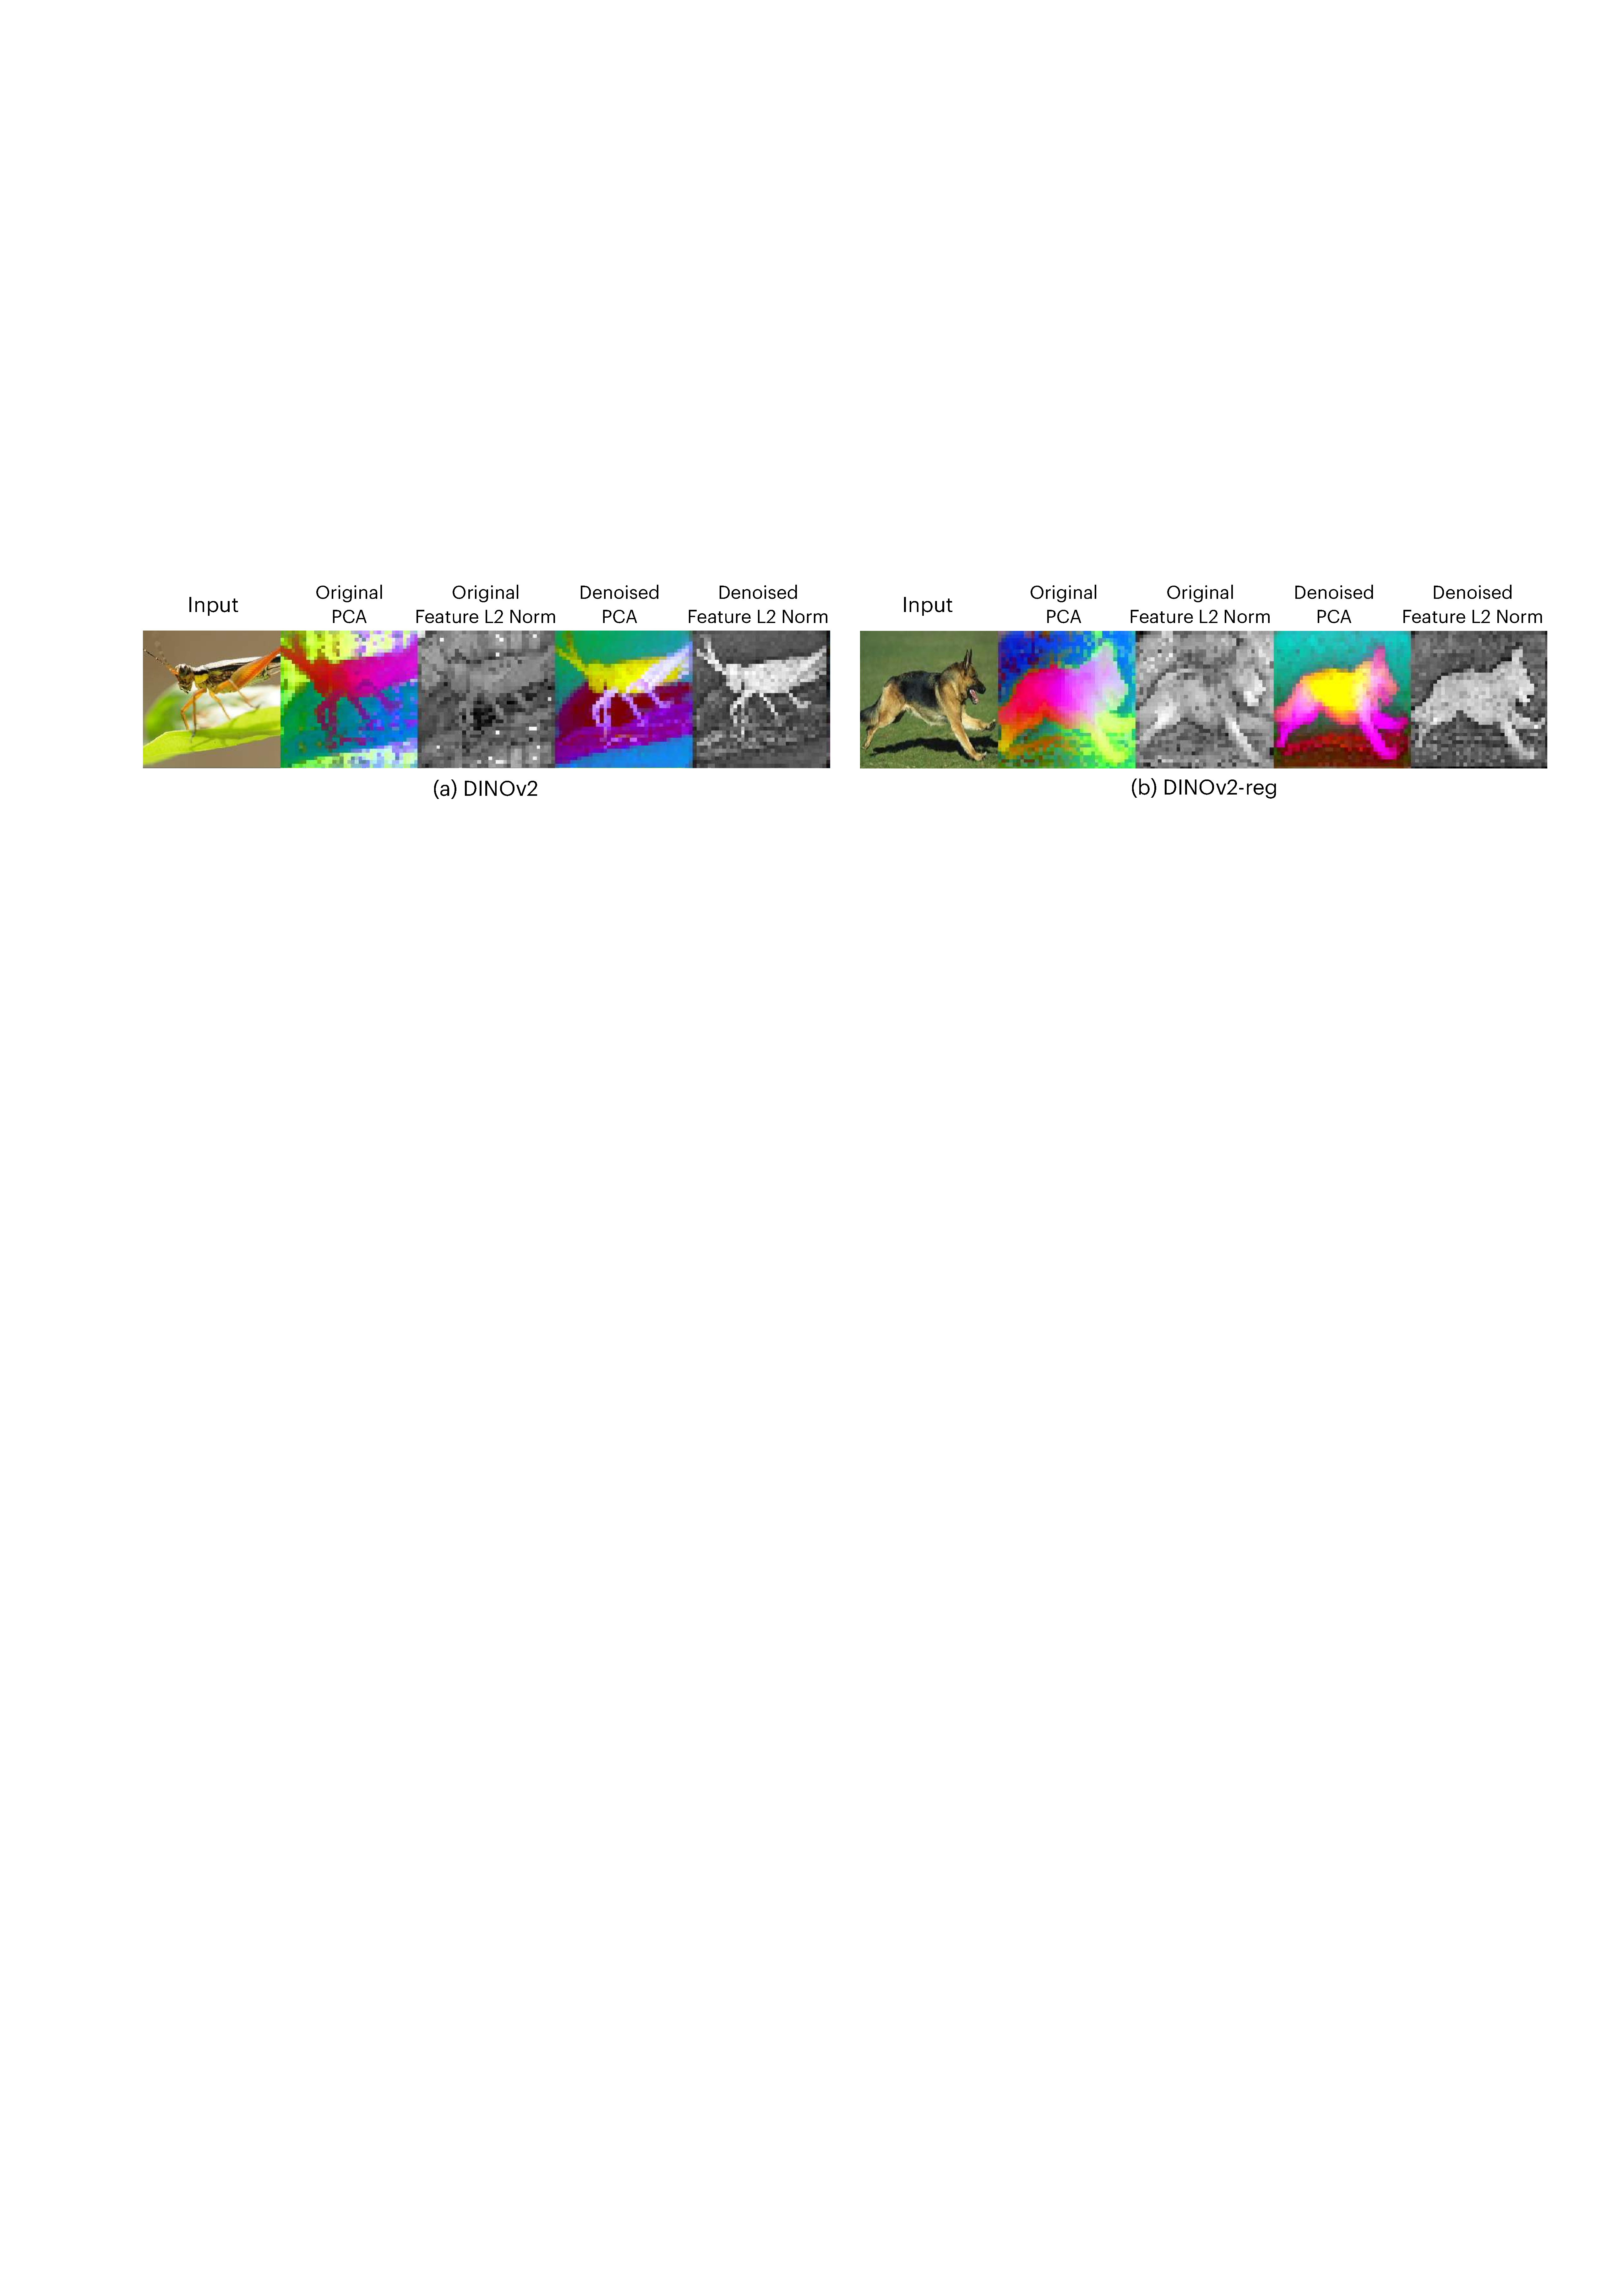
\includegraphics[width=1\linewidth]{figures/fig6_emerging_obj_dis.pdf}
    \caption{\textbf{Emerged object discovery ability.} The features denoised by our \ours show higher feature norms on objects of interest.}
    \label{fig:emerg_obj_dis}
\end{figure}
%##################################################################################################

%##################################################################################################
\begin{table*}[t!]
    \centering
    \caption{\textbf{Unsupervised object discovery using LOST \cite{simeoni2021localizing}.} We report the corloc score across three datasets. Our \ours significantly improves existing models. $^\dagger$: results quoted from \cite{darcet2023vision}; these models are ViT-\textit{large} trained on the ImageNet-22k dataset while our reported results are based on the publicly available ViT-\textit{base}.}
    \tablestyle{3.5pt}{1.2}
    \begin{tabular}{l | y{50} y{50} y{50}}
        Method                                                & VOC2007                                     & VOC2012                                     & COCO20k                                     \\
        \shline
        (a) \gc{$^\dagger$DINOv2} \cite{oquab2023dinov2}   & \gc{35.3}                                   & \gc{40.2}                                   & \gc{26.9}                                   \\
        (b) \gc{$^\dagger$DINOv2-reg} \cite{darcet2023vision} & \gc{55.4}                                   & \gc{60.0}                                   & \gc{42.0}                                   \\
        \hline
        (c) DINOv2-reg                                        & 38.0                                        & 41.5                                        & 26.9                                        \\
        \baseline{(d) DINOv2-reg + \textbf{\ours}}            & \baseline{\textbf{56.1} \increase{(+18.1)}} & \baseline{\textbf{59.3} \increase{(+17.8)}} & \baseline{\textbf{45.5} \increase{(+18.6)}} \\
        \hline
        (e) DINOv2                                            & 30.8                                        & 35.9                                        & 23.4                                        \\
        \baseline{(f) DINOv2 + \textbf{\ours}}                & \baseline{\textbf{58.0} \increase{(+27.2)}} & \baseline{\textbf{60.3} \increase{(+24.4)}} & \baseline{\textbf{46.7} \increase{(+23.3)}} \\
    \end{tabular}
    \label{tab:obj_discovery}
\end{table*}
%##################################################################################################

\paragraph{Object discovery.} Unsupervised object discovery has been a long-standing problem of interest. An intriguing finding from our experiments is the emerging capability of object discovery in denoised ViTs. \cref{fig:emerg_obj_dis} illustrates this through PCA visualizations and $L2$ norms of the feature maps. Post-denoising, not only are the artifacts removed, but also the objects of interest become more distinctly visible from the feature norm values. This enhancement in object clarity is \textit{not} a goal of \ours but emerges as the outcome of our method.

To quantitatively assess these enhancements, we follow \cite{darcet2023vision} to use LOST \cite{simeoni2021localizing} for evaluating object discovery efficacy before and after applying our \ours. We use feature norms as an indicator of object prominence. We conduct object discovery experiments on PASCAL VOC 2007 \cite{pascal-voc-2007} and 2012 \cite{pascal-voc-2012} and COCO20k datasets \cite{lin2014microsoft}.
\cref{tab:obj_discovery} presents the results. Our \ours significantly improves both DINOv2 \cite{oquab2023dinov2} and DINOv2-reg \cite{darcet2023vision} in all the evaluated datasets. In particular, while the publicly available DINOv2-reg shows some improvements ((c) \textit{vs.} (e)), we find that it falls short of the performance levels reported in \cite{darcet2023vision} ((c) \textit{vs.} (b)). Despite this, our \ours achieves more substantial enhancements in object discovery capabilities, even compared to the numbers reported in \cite{darcet2023vision} ((f) \textit{vs.} (b)).



%##################################################################################################
\noindent
{
    \begin{minipage}[t]
        {0.41\textwidth}
        \centering
        \small
        \makeatletter\def\@captype{table}\makeatother\caption{Ablation study on per-image denoising using KNN segmentation protocol on VOC12\texttt{val}.}
        \tablestyle{3.5pt}{1.2}
        \begin{tabular}{l | x{40}}
            Representations                                           & mIoU                      \\
            \shline
            (a) DINOv2                                                & 65.35                     \\
            \hline
            (b) $\mathcal{F}$                                         & 67.81                     \\
            (c) $\mathcal{F} + \mathcal{G}$                           & 70.82                     \\
            \baseline{(d) $\mathcal{F} + \mathcal{G} + \hat{\Delta}$} & \baseline{\textbf{70.94}} \\
        \end{tabular}
        \label{tab:per_img_denoising}
    \end{minipage}
    \quad
    \begin{minipage}[t]{0.53\textwidth}
        \centering
        \small
        \makeatletter\def\@captype{table}\makeatother\caption{Ablation study on the architectural design of generalizable denoiser. We report the mIoU of the VOC2012 validation set.}
        \tablestyle{3.5pt}{1.2}
        \begin{tabular}{l | x{40}}
            Denoiser architectures                        & mIoU                      \\
            \shline
            (a) DINOv2 (reproduced)                       & 83.60                     \\
            \hline
            (b) conv1x1                                   & 82.15                     \\
            (c) conv3x3                                   & 83.27                     \\
            \baseline{(d) Single Transformer Block + PE.} & \baseline{\textbf{84.84}} \\
            (e) Single Transformer Block                  & 84.81                     \\
        \end{tabular}
        \label{tab:denoiser}
    \end{minipage}
}
%##################################################################################################

\subsection{Ablation Study}
In this section, we provide ablation studies to understand the importance of different components in our proposed \ours.

\paragraph{Factorization.} We ablate our per-image denoising method using a K-Nearest-Neighbor (KNN) pixel segmentation evaluation protocol on the VOC2012 dataset. Specifically, we collect class centroids from each training image by masked pooling to construct a memory bank using ground truth annotations. Then, for each pixel in a validation image, we classify it based on its 20 nearest neighbors in the memory bank. We report the mIoU on the validation set. \cref{tab:per_img_denoising} shows the results. We observe that combining the artifact field $\mathcal{G}$ and the residual term $\hat{\Delta}$ yields the best result (d). Omitting both these elements reduces our approach to merely utilizing a neural field $\mathcal{F}$ to learn multi-crop ensembled image features, without addressing artifacts (b). While this variant shows improvement, it falls behind our proposed method by a large margin, underscoring the importance of removing artifacts.

\paragraph{Generalizable denoiser.} We explore alternative architectural designs for our generalizable denoiser in \cref{tab:denoiser}. We study four variations: 1) our default setting, which incorporates a single Transformer Block with new learnable position embeddings; 2) our default setting but without position embeddings; 3) a multi-layer convolution denoiser with a \texttt{Conv1x1-ReLu-Conv1x1-ReLu-Conv1x1} structure, and 4) a multilayer convolution denoiser with a \texttt{Conv3x3-ReLu-Conv3x3-ReLu-Conv3x3} structure. We observe that denoisers based on convolutional structures (b, c) do not yield good results, with the conv1x1 setting performing the worst (c).
Moreover, we note that our default setting with a Transformer block and learnable positional embeddings achieves the best result (d), and removing the learnable position embeddings obtains very similar numerical performance (e). We empirically find that the design of (d) leads to better qualitative visualizations, and thus we use this setting.


%##################################################################################################
\begin{figure}[t!]
    \centering
    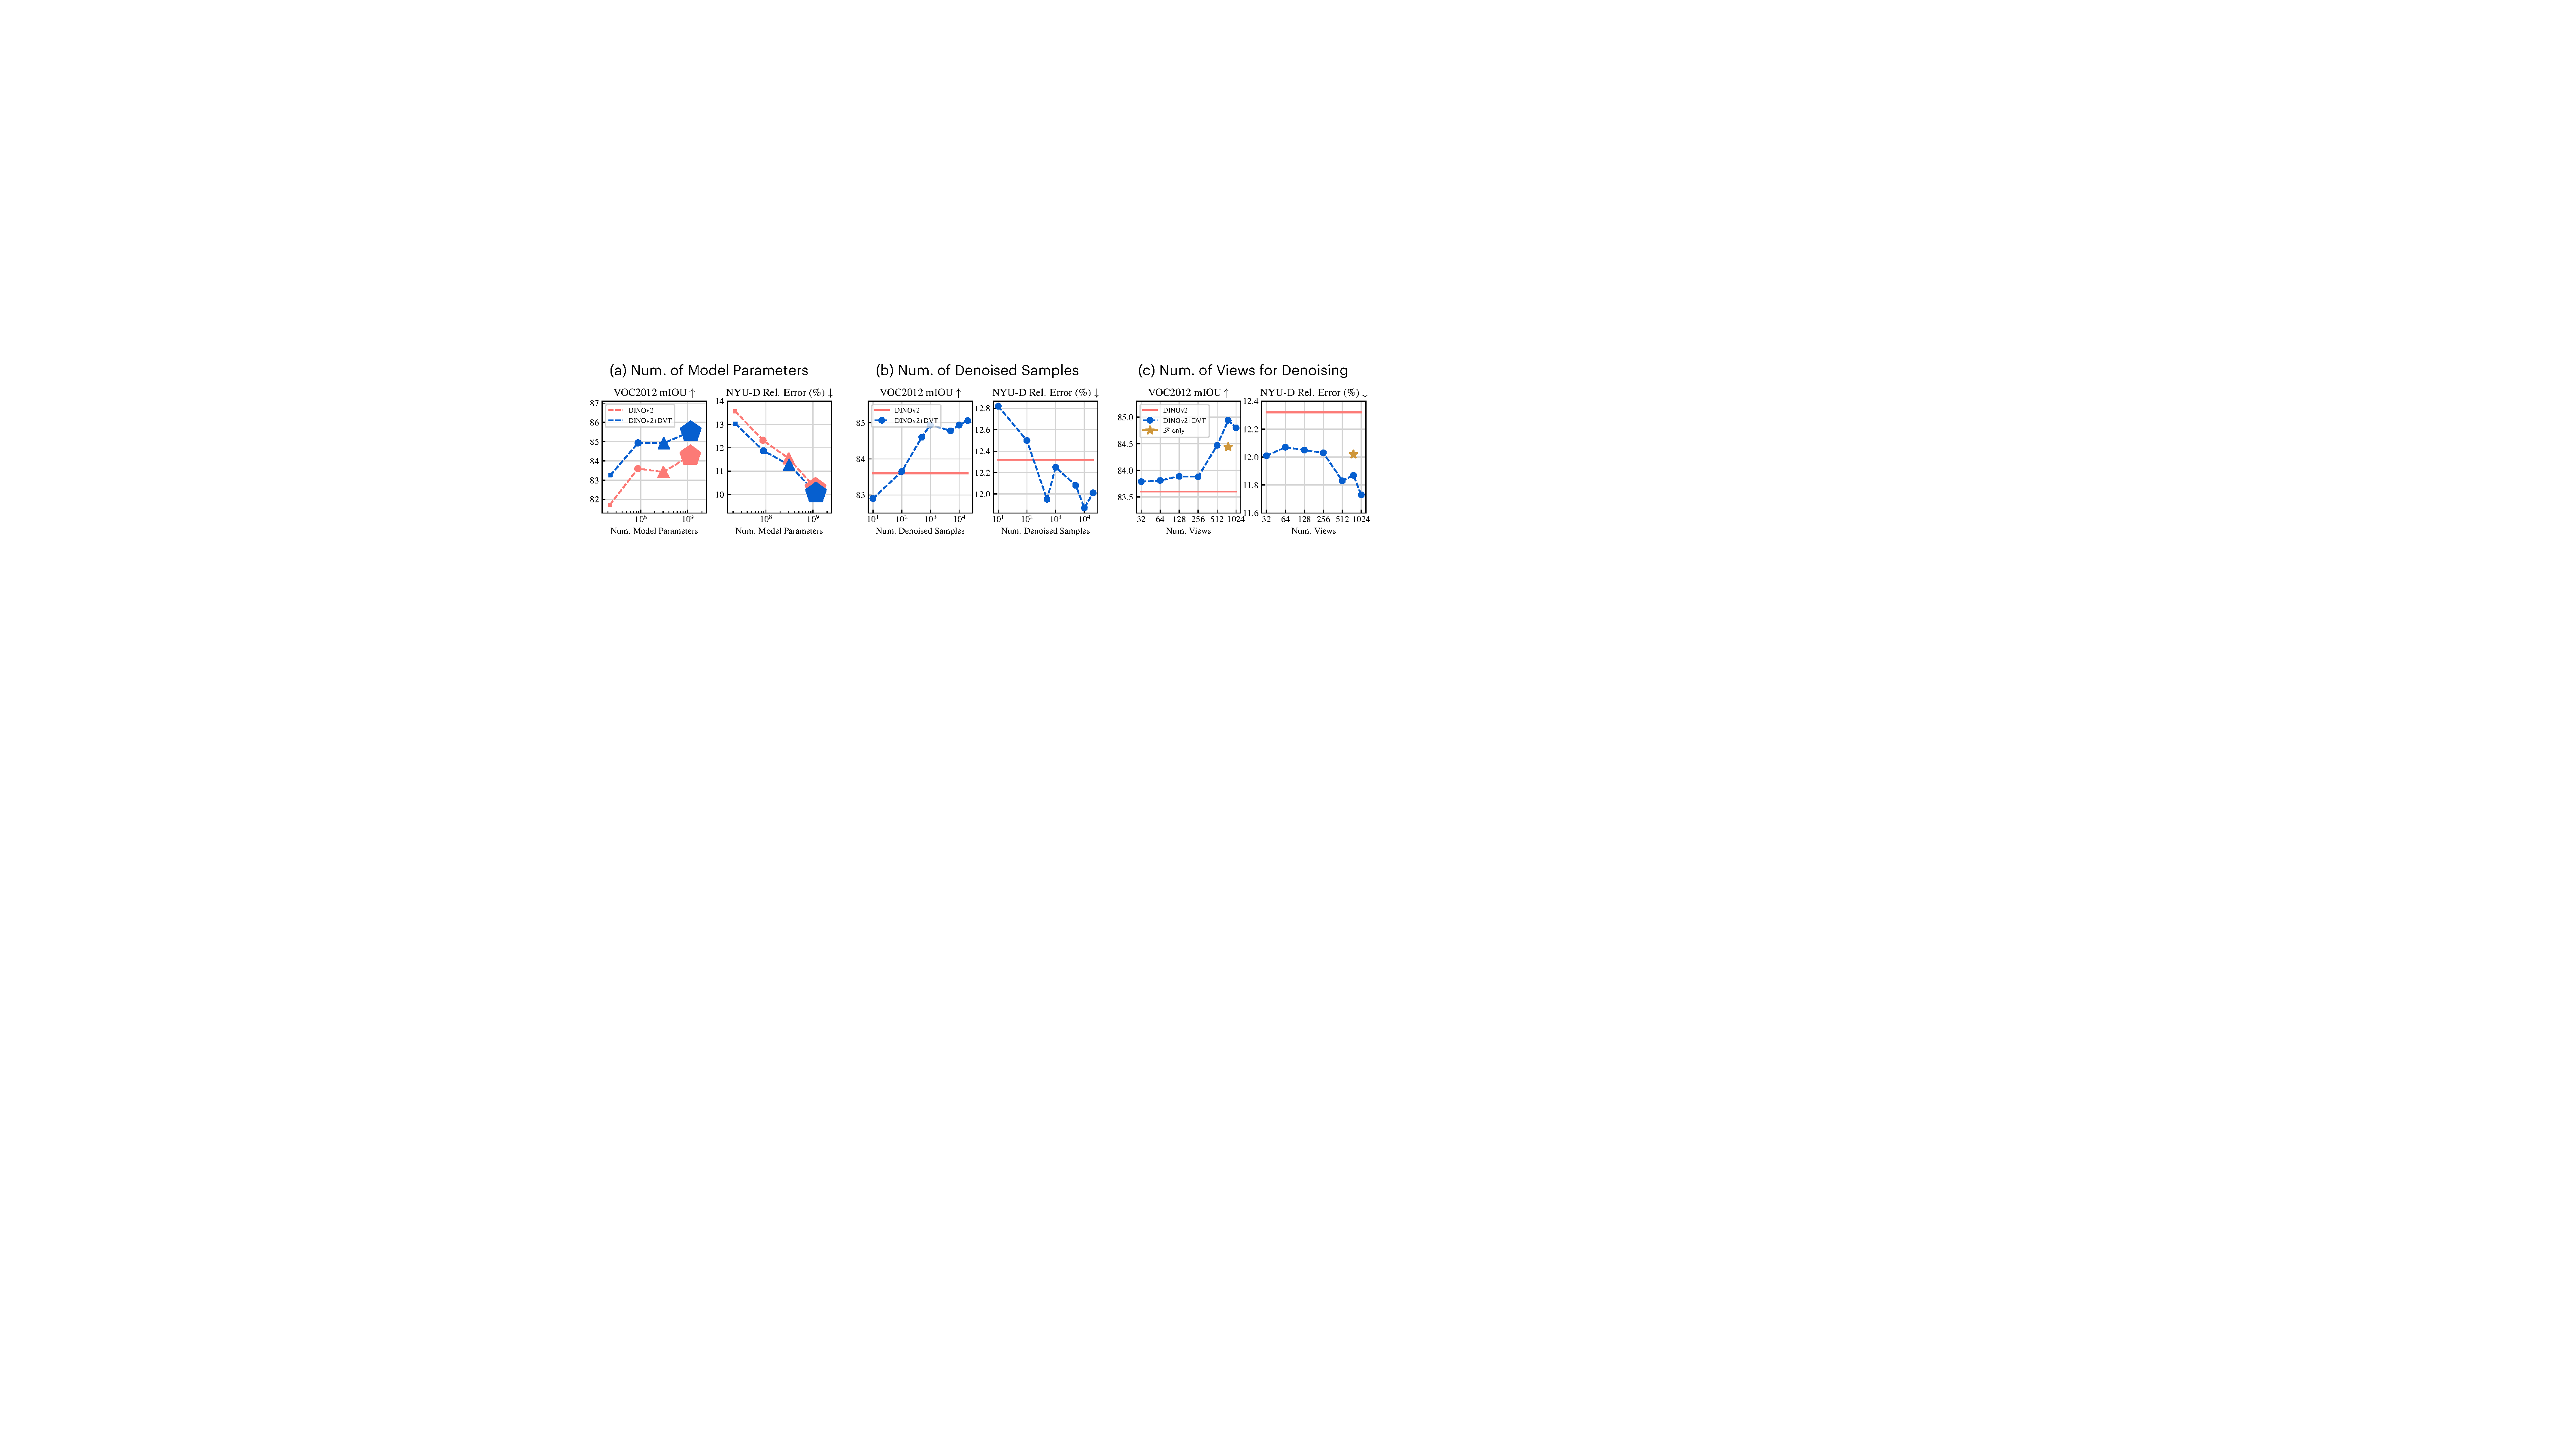
\includegraphics[width=1\linewidth]{figures/fig7_ablation.pdf}
    \caption{\textbf{DVT's Scaling Behaviors.} We study the generalizable denoiser's performance for (a) different model sizes, (b) the number of denoised samples used for training denoisers, and (c) the number of views used when performing per-image denoising.}
    \label{fig:scaling}
\end{figure}
%##################################################################################################

\paragraph{Scaling behaviors.} We study how \ours scales with model sizes and data scales in \cref{fig:scaling}. In (a), we see \ours boosts differently-sized ViTs, even allowing ViT-\textit{base} to match or exceed ViT-\textit{giant} performance in semantic segmentation. Overall, \ours's scaling behaviors closely align with those of baseline models. In (b), we study the impact of the number of denoised training samples on task performance, where \ours shows promising results even with limited training samples (\eg, 100$\sim$1000). Note that our denoiser never sees ADE20k and NYU-depth datasets during training, yet generalizes effectively.
In (c), we plot the task performance \vs the number of views used for the denoising. \ours benefits from more views in first-stage denoising. When training neural fields, more views enhance performance, while fewer views lead to overfitting.
In particular, aggregating views is itself an approach to denoising, which still \textit{aligns with} our motivation.
We also demonstrate that a denoiser trained on samples denoised solely by aggregating views via neural fields (${\mathcal{F}}$-only in (c)) surpasses baselines but underperforms the full \ours, which further confirms the effectiveness of our proposed denoising procedure.

